%% ------------------------------------------------------------------------- %%
\chapter{Cronograma}
\label{cap:cronograma}

\section{Próximos passos}

A proposta deste trabalho é avaliar o uso das redes convolucionais no problema de \textit{code retrieval}. Conforme \cite{Goodfellow-et-al-2016:pratical-methodology}, o primeiro passo é definir um objetivo, um valor alvo para o modelo. No nosso caso, o objetivo é obter um resultado comparável ao modelo proposto por \cite{cambronero-deep-learning-code-search:2019}, que é o estado da arte atualmente.

O processo de treinamento de uma rede neural envolve algumas etapas. Desde o processo de tomada de decisão para uso de deep learning, coleta dos dados, seleção da arquitetura, treinamento e avaliação do modelo. Algumas etapas foram parcialmente concluídas durante o estudo preliminar. A figura~\ref{fig:neural-network-process-training} abaixo ilustra as etapas do processo de treinamento e o andamento através de um mapa de calor. A tabela~\ref{table:etapas-processo-treinamento} lista as principais atividades em andamento e/ou concluídas.


\begin{figure}[h]
    \centering
    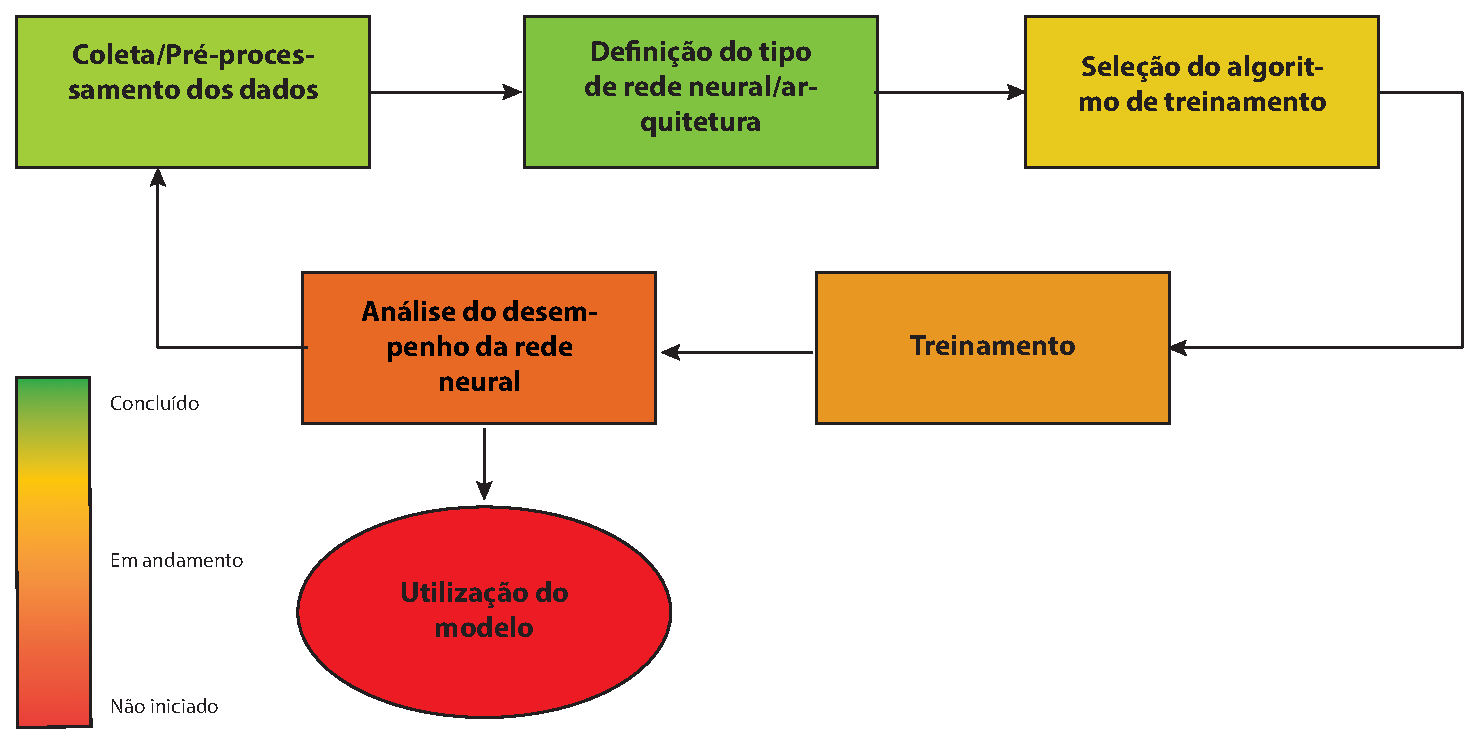
\includegraphics[width=1\textwidth]{figuras/cap-cronograma/training_process.pdf}
    \caption{Etapas do processo de treinamento de uma rede neural. As etapas de \emph{Análise do desempenho da rede neural} e \emph{Treinamento} estão no início. Enquanto a \emph{Coleta/Pré-processamento dos dados} e \emph{Definição do tipo de rede neural/arquitetura} estão parcialmente concluídas. Figura adaptada do livro \cite{nndesign:2014:pratical-training-issues}}
    \label{fig:neural-network-process-training}
\end{figure}

{\footnotesize
\centering
\begin{longtable}{ p{8em} p{8em} p{10em} p{8em} p{6em} }
%\centering
%\begin{tabular}{ p{10em} p{10em} p{10em} p{6em} }
\hline
\textbf{Etapa} & \textbf{Atividade} & \textbf{Tarefa} & \textbf{Forma de avaliação} & \textbf{Status} \\
\hline
Coleta/Pré-processamento dos dados & Utilização dos dados coletados por \cite{yao-2018} & & & Concluído  \\
\hline

Coleta/Pré-processamento dos dados & Pré-processamento dos dados & Verificar a possibilidade de quebra das palavras do código-fonte de acordo com a convençao de nomenclatura (\textit{snake case}). E analisar a possibilidade de remoção de \textit{stop words} & Análise das curvas de erros de validação e treinamento. Melhora da métrica MRR. & Parcialmente concluído  \\
\hline

Coleta/Pré-processamento dos dados & Treinamento não-supervisionado: \textit{word2vec} & Análise do vetor de representação distribuída e se há necessidade de ajustes nos parâmetros de treinamento e dimensão do vetor & Visualização do t-SNE para as 50 palavras mais frequentes das questões e trechos de código-fonte e suas relações. & Parcialmente concluído  \\
\hline

Definição do tipo de rede neural/arquitetura & Modelo proposto: CNN & & & Concluído  \\
\hline

Definição do tipo de rede neural/arquitetura & Modelos para comparação: \textit{Embedding} e o \textit{bi-modal embedding} com o mecanismo de atenção proposto por \cite{cambronero-deep-learning-code-search:2019} & Implementar o modelo proposto por \cite{cambronero-deep-learning-code-search:2019} & & Em andamento  \\
\hline

Definição do tipo de rede neural/arquitetura & Definição do objetivo: Resultado comparável ao modelo proposto por \cite{cambronero-deep-learning-code-search:2019} em um mesmo ambiente de testes e conjunto de dados & Inicialmente, buscamos um desempenho superior em pelo menos 10p.p. em relação ao modelo do \cite{cambronero-deep-learning-code-search:2019}. Dependendo do desempenho do nosso modelo, este valor alvo pode ser revisto & MRR & Em andamento  \\
\hline

Definição do tipo de rede neural/arquitetura & Seleção dos hiper-parâmetros do modelo & Esta tarefa será feita em conjunto com o treinamento. Conforme o desempenho do modelo, ajustes nos hiper-parâmetros devem ser feitos para aumentar ou diminuir a capacidade do modelo & Análise da curva de erro de validação e treinamento vs capacidade do modelo & Em andamento  \\
\hline

Seleção do algoritmo de treinamento & Algoritmo de otimização para o modelo & Inicialmente, utilizamos o algoritmo de otimização Adam para o modelo. Uma alternativa é verificar o desempenho para outros algoritmos como SGD e RMSprop & Análise da curva de erro de validação e treinamento vs época & Parcialmente Concluído  \\
\hline

Treinamento & Regularização & Utilizar técnica de regularização \textit{dropout} ou \textit{batch normalization} & Análise da curva de erro de validação e treinamento vs época & Não iniciado  \\
\hline

Treinamento & Função objetivo & Função de perda \textit{hinge} &  & Concluído  \\
\hline

Treinamento & Critério de parada & Adotamos os mesmos critérios de treinamento proposto por \cite{iyer-etal-2016-summarizing}. O treinamento é feito durantes 80 épocas ou enquanto o erro for maior que um certo valor. No caso, estamos utilizando o valor $0,001$ & & Concluído  \\
\hline

Análise do desempenho da rede neural & \textit{Overfitting} e extrapolação & Diminuir a diferença entre o erro de validação e o erro de treinamento do modelo CNN. Inicialmente, utilizaremos técnicas de regularização e algortimos de otimização.  & Análise através das curvas de erro de validação e treinamento vs época e capacidade do modelo & Em andamento \\
\hline

Análise do desempenho da rede neural & Visualização do pior caso & Analisar as classificações feita pelo modelo através dos piores casos. No nosso caso, os piores casos são os trechos com os menores valores de MRR. Conforme \cite{Goodfellow-et-al-2016:pratical-methodology}, esta análise permite identificar possíveis problemas no conjunto de dados. & Verificação manual & Em andamento \\
\hline

Análise do desempenho da rede neural & Avaliação manual & Avaliar manualmente uma amostra de questões e trechos de código-fonte classificados pelos modelos & Verificação manual & Em andamento \\
\hline

Uso do modelo & Busca & Coletar ou propor novas questões ao modelo e avaliar as respostas. Verificar também o desempenho do modelo na busca por trechos similares em um corpus de busca diferente, e.g., Github & Verificação manual & Não iniciado \\
\hline

 
%\end{tabular}
\caption{Relação das principais atividades realizadas e a serem cumpridas neste trabalho.}
\label{table:etapas-processo-treinamento}
\end{longtable}}


\section{Cronograma}

O processo de treinamento de um modelo é um ciclo, conforme a figura~\ref{fig:neural-network-process-training}. Para facilitar o acompanhamento do progresso do trabalho, preferimos definir alguns marcos a serem alcançados até a entrega. Os marcos que julgamos importantes são:

\begin{enumerate}
\item Implementação do modelo proposto por \cite{cambronero-deep-learning-code-search:2019}

\item Adição de regularização aos modelos

\item Avaliação dos piores casos

\item Avaliação manual

\item Compilação dos resultados

\item Submissão de um artigo com os resultados em um congresso internacional

\end{enumerate}

O cronograma dos próximos passos pode ser visualizado através da figura~\ref{fig:cronograma-proximos-passos-gantt-chart}.

\begin{figure}[h]
    \centering
    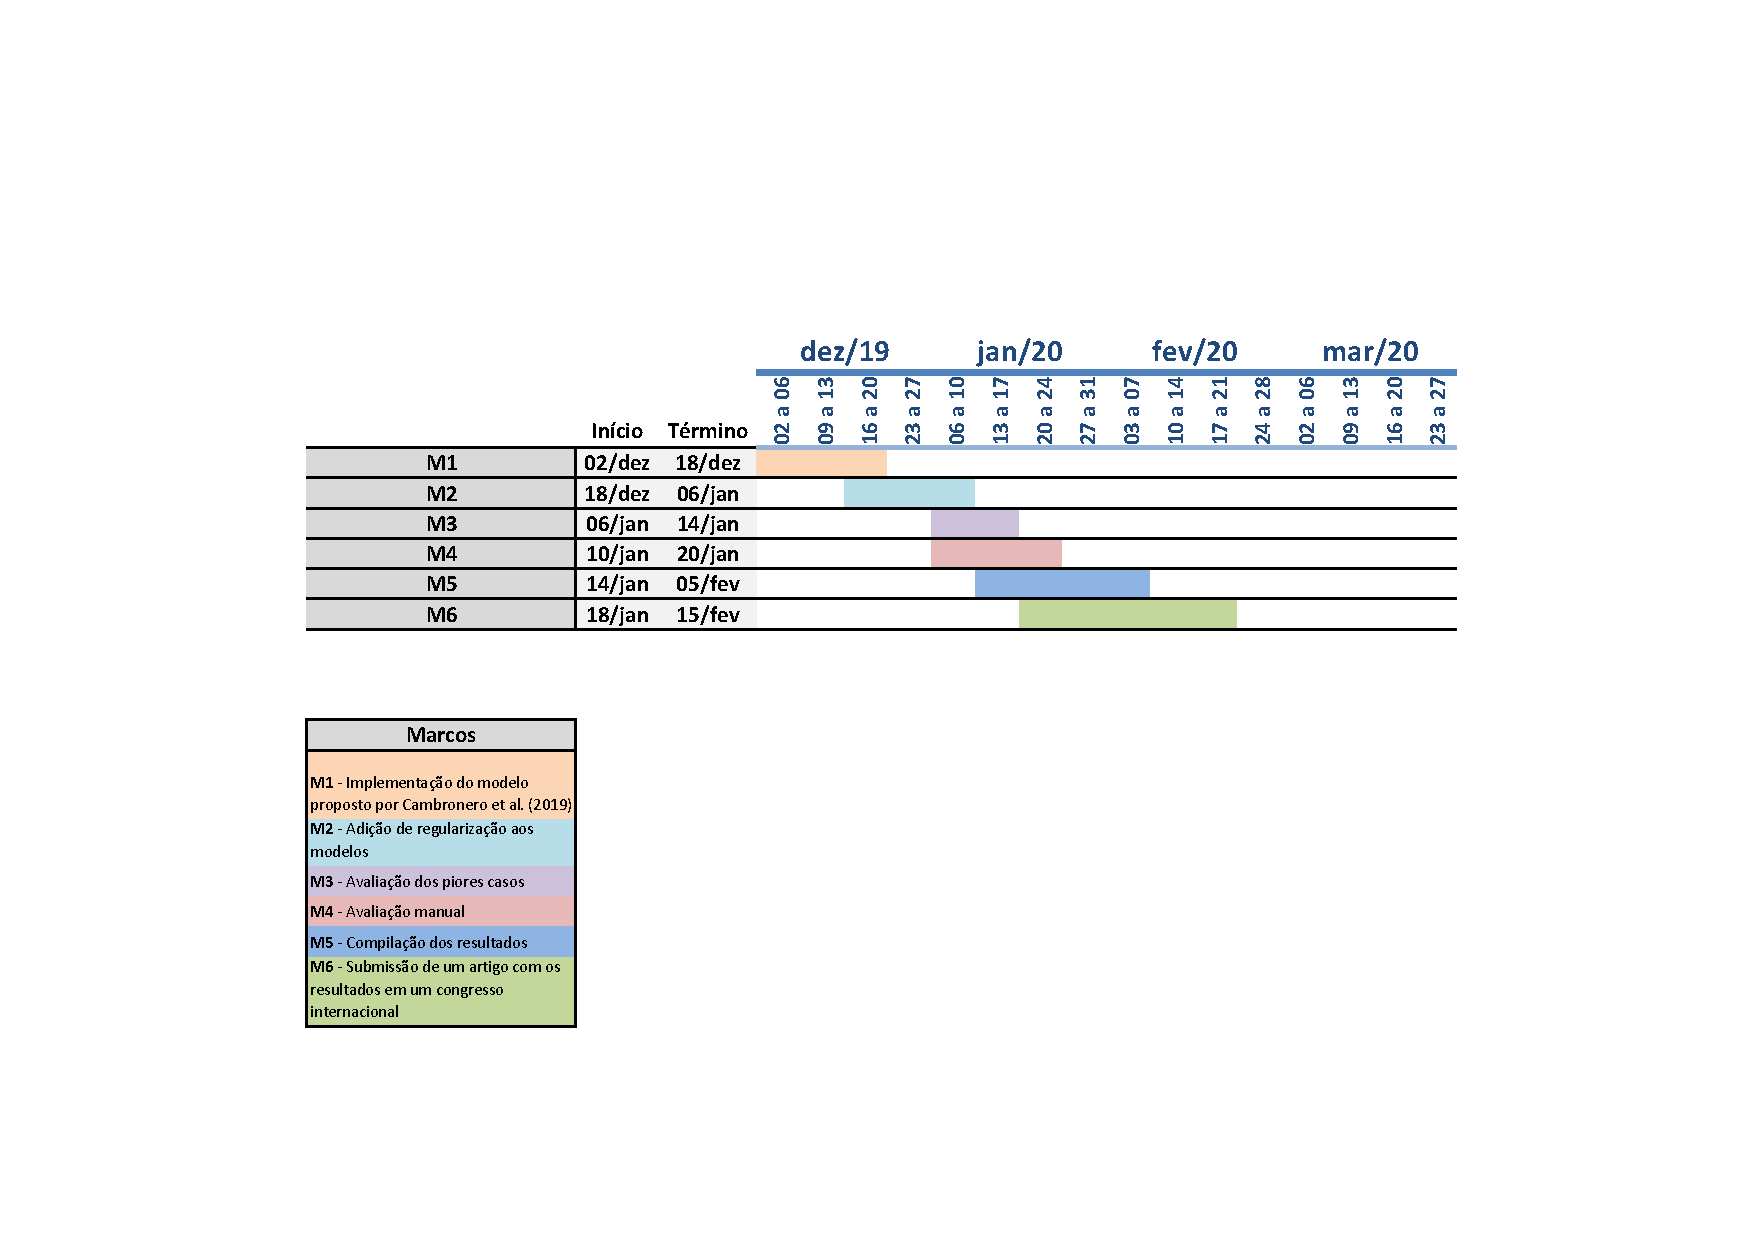
\includegraphics[width=1\textwidth]{figuras/cap-cronograma/cronograma_trabalho.pdf}
    \caption{Cronograma dos próximos passos até a entrega do trabalho}
    \label{fig:cronograma-proximos-passos-gantt-chart}
\end{figure}



